\documentclass{beamer}
\usetheme{Boadilla}
\usepackage[T1]{fontenc}

\title{Redundantny system plików}

\author{Kacper Pieniążek}
\date{\today}

\begin{document}
	\begin{frame}
		\titlepage
	\end{frame}

	\section{Section 1}
	\subsection{sub a}
	
	\begin{frame}
		\frametitle{Cel pracy}
			System plików zapewniający ochronę danych nawet w przypadku ich uszkodzenia w oparciu o interfejs FUSE.
	\end{frame}

	\begin{frame}
		\frametitle{Założenia pracy}
		\begin{itemize}
			\pause
			\item Wykrywanie niezgodności danych
				\begin{itemize}
					\item Sumy kontrolne
					\item Kody korekcyjne
				\end{itemize}
			\pause
			\item Odzyskiwanie danych
			\begin{itemize}
				\item Duplikacja danych
				\item Kody korekcyjne
			\end{itemize}
			\pause
			\item Obsługa wybranych funkcjonalności systemu plików
			\begin{itemize}
				\item Pełna funkcjonalność, jeśli jest aktywna replika typu 1.
			\end{itemize}
			\pause
			\item Wygodne użytkowanie
			\begin{itemize}
				\item Podział i duplikacja danych wystarczająco transparentna dla użytkownika
				\item Rozwiązywanie konfliktów w przypadku niezgodności danych
				\item Dostosowanie systemu do własnych potrzeb
			\end{itemize}
		\end{itemize}
	\end{frame}
	
	\begin{frame}
		\frametitle{Analiza problemu}

		\begin{itemize}
			\item Jak zapewnić redundancję?
			\pause
			\item Jak zapewnić spójność danych?
			\begin{itemize}
				\item W przypadku braku synchronizacji między replikami, wybór poprawnych danych
			\end{itemize}
			\pause
			\item Jak wykrywać rozbieżność danych?
			\begin{itemize}
				\item Podczas operowania na uszkodzonych danych; błędny odczyt, kody korekcyjne, sumy kontrolne 
			\end{itemize}
			\pause
			\item Jak naprawiać rozbieżność danych?
			
		\end{itemize}
	\end{frame}
		
	\begin{frame}
		\frametitle{Rozwiązanie}
			\begin{block}{Definicja}
				Replika - jeden z podsystemów zawierający kopię chronionych danych
			\end{block}
			\pause
			\begin{itemize}
				\item Cały system może być podzielony na warstwy współpracujące ze sobą. 
				\begin{itemize}
					\item Każda replika to nowa warstwa
				\end{itemize}
				\pause
				\item Podział na warstwy umożliwia rozwiązania typu RAID
			\end{itemize}
			
	\end{frame}

		
\begin{frame}
	\frametitle{Rozwiązanie}
	\begin{block}{Definicja}
            Repliki standardowe zapewniają redundancję, synchronizację oraz podział danych
	\end{block}
	\pause
	\begin{block}{Definicja}
	        Repliki korecyjne zapewniają korekcję błędów oraz więcej sposobów ich detekcji.
    \end{block}
\end{frame}

\begin{frame}
        \frametitle{Replika blokowa (BR)}
		\begin{columns}
		\column{0.7\textwidth}
		\begin{block}{Redundancja}
			Standardowa replika blokowa nie zapewnia ochrony danych, jedynie ich rozkład w warstwie
		\end{block}
		\begin{itemize}
			\item Podstawa do pozostałych replik blokowych
			\item Dwa podziały:
			\begin{itemize}
				\item Bloki stałej długości
				\item Bloki zmiennej długości
			\end{itemize}
			\item Operacje read, write, open, close, stat

			\item Podział danych niewidoczny dla użytkownika
		\end{itemize}
		\column{0.3\textwidth}
		\begin{figure}
			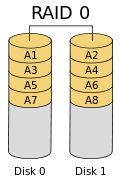
\includegraphics[scale=0.5]{raid-0.png}
		\end{figure}
		\end{columns}
\end{frame}

\begin{frame}
    \frametitle{BR o stałej ilości bloków}
    \begin{figure}[h!]
            \centering
            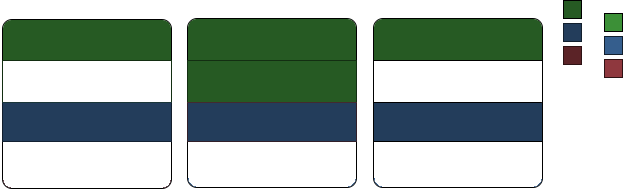
\includegraphics[scale=0.6]{BR-1.png}
            \caption{Replika blokowa na trzech katalogach}
            \label{fig:br1}
    \end{figure}
\end{frame}

\begin{frame}
    \frametitle{BR o zmiennej ilości bloków}
    \begin{figure}[h!]
            \centering
            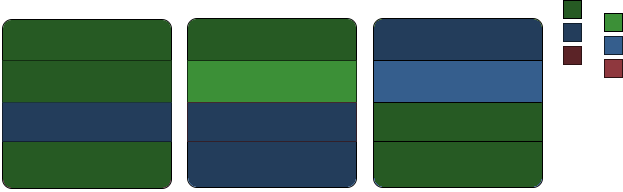
\includegraphics[scale=0.6]{BR-2.png}
            \caption{Replika blokowa na trzech katalogach}
            \label{fig:br2}
    \end{figure}
\end{frame}


\begin{frame}
        \frametitle{Replika lustrzana (MR)}
	\begin{columns}
		\column{1.0\textwidth}
		\begin{block}{Redundancja}
                Standardowa MR tworzy odbicie lustrzane danych, zapewnia funkcjonalność równą systemu nadrzędnego
		\end{block}
		\begin{itemize}
			\item Wysoki koszt pamięci
			\item Pełna funkcjonalność systemu plików
			\item Uszkodzone dane zastąpione danymi z odbicia
		\end{itemize}
	\end{columns}
\end{frame}
	

\begin{frame}
        \frametitle{Replika lustrzana (MR)}
	\begin{columns}
		\column{1.0\textwidth}
		\begin{figure}
			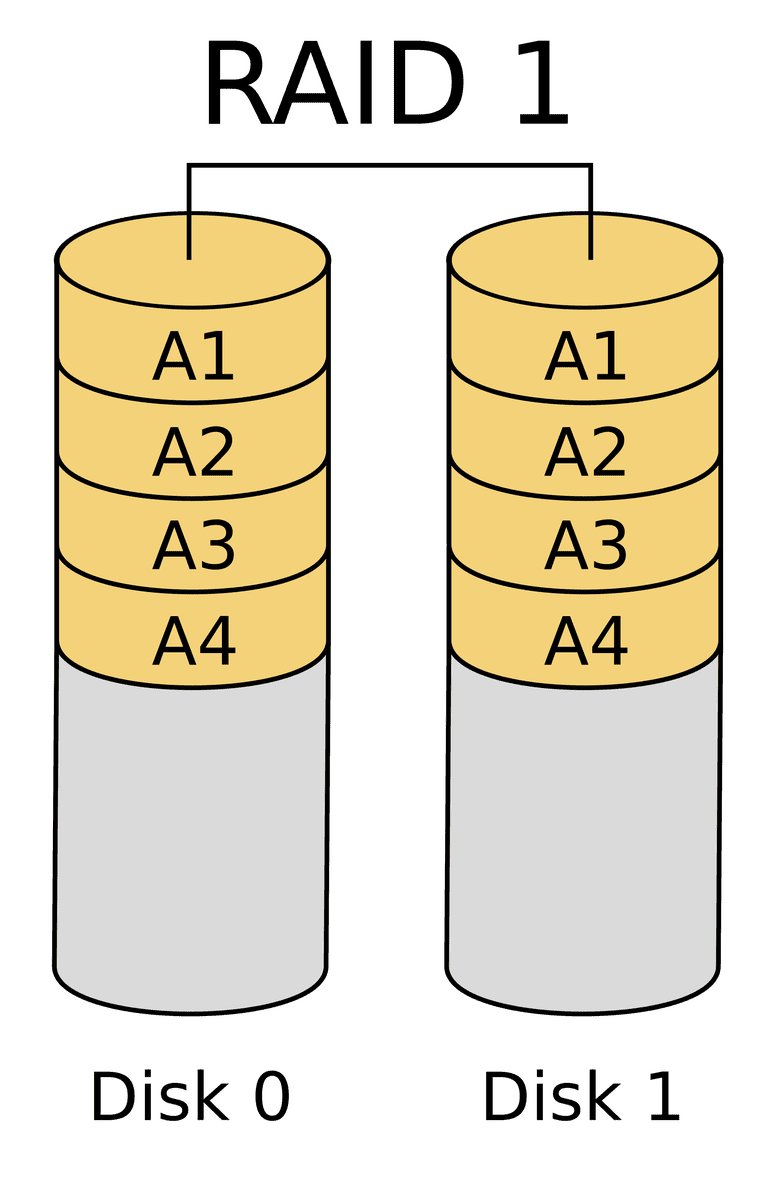
\includegraphics[]{raid-1.png}
		\end{figure}
	\end{columns}
\end{frame}
	
\begin{frame}
        \frametitle{Repliki korekcyjne }
	\begin{columns}
		\column{1.0\textwidth}
		\begin{block}{Korekcja błędóww}
		   Repliki korekcyjne są w stanie naprawiać własne błędy podczas operacji lub synchronizacji z innymi replikami.
        \end{block}
		\begin{itemize}
			\item Kod Hamminga 
			\item Bloki parzystości
			\item Kod Reeda-Solomona
		\end{itemize}
	\end{columns}
\end{frame}
			
	\begin{frame}
		\frametitle{Przykłady}
		\begin{block}{Przykład}
			Dysk, na którym zamontowana była jedna z replik lustrzanych dane został odłączony. 
		\end{block}
		\pause
		\begin{block}{Przykład}
			Wystąpił błąd poczas zapisu do jednej z replik blokowych.
		\end{block}
		\pause
		\begin{block}{Przykład}
			Obrócone bity na danych w jednej z replik.
		\end{block}
	\end{frame}
	

	\begin{frame}
		\frametitle{Ulepszenia}
		\begin{itemize}
			\item Kolejne warstwy
			\item Usprawnienie działania
			\begin{itemize}
				\item Wykorzystanie wywołań niskiego poziomu FUSE
				\item Optymalizacja zastosowanych operacji
			\end{itemize}
			\item Implementacja całej funkcjonalności systemu plików dla pozostałych warstw
			\item Pełna niewidoczność działania systemu dla użytkownika
		\end{itemize}
	\end{frame}

\end{document}
